% =====================================================================
% Engineering Examples
% ---------------------------------------------------------------------
% Examples for the packages loaded in Base Packages.tex that are most
% useful in engineering reports: siunitx, amsmath, pgfplots, circuitikz,
% tikz, listings and cite. Delete whatever you do not need.
% =====================================================================

\section{Engineering Examples}
\label{sec:engineering}

\subsection{Units and Numbers}

Always write quantities with \texttt{siunitx} instead of typing units by
hand. It handles spacing, upright units and number formatting for you.
The template sets it up for IEEE style in \texttt{Base Packages.tex}: a
regular space before the unit, a slash for ``per'', a centre dot between
units, the unit written once in ranges and lists, and no space before
\%.

\begin{table}[H]
    \centering
    \caption{Common \texttt{siunitx} commands}
    \label{tab:siunitx-commands}
    \begin{tabular}{ll}
        \toprule
        Source & Output \\
        \midrule
        \verb|\qty{9.81}{\metre\per\second\squared}| & \qty{9.81}{\metre\per\second\squared} \\
        \verb|\qty{4.7}{\kilo\ohm}|                  & \qty{4.7}{\kilo\ohm} \\
        \verb|\qty{1.2e-3}{\farad}|                  & \qty{1.2e-3}{\farad} \\
        \verb|\num{123456.789}|                      & \num{123456.789} \\
        \verb|\qtyrange{10}{50}{\hertz}|             & \qtyrange{10}{50}{\hertz} \\
        \verb|\qtylist{1;2;5}{\milli\metre}|         & \qtylist{1;2;5}{\milli\metre} \\
        \verb|\qtyproduct{2 x 5}{\centi\metre}|      & \qtyproduct{2 x 5}{\centi\metre} \\
        \verb|\qty{20}{\percent}|                   & \qty{20}{\percent} \\
        \verb|\qtyrange{20}{30}{\percent}|          & \qtyrange{20}{30}{\percent} \\
        \verb|\unit{\newton\metre}|                  & \unit{\newton\metre} \\
        \verb|\ang{45}|                              & \ang{45} \\
        \verb|\qty{20}{\celsius}|                    & \qty{20}{\celsius} \\
        \bottomrule
    \end{tabular}
\end{table}

\subsection{Multi-line Equations}

Use \verb|align| for derivations. Put \verb|&| before the symbol to line up
on, end each line with \verb|\\|, and label only the lines you will
reference (use \verb|\nonumber| on the others). \Cref{eq:power-final} is
derived from \cref{eq:ohm,eq:power}.
\begin{align}
    P &= VI \nonumber \\
      &= (IR)\,I \nonumber \\
      &= I^2 R \label{eq:power-final}
\end{align}

Matrices are written with \verb|bmatrix|. \Cref{eq:state-space} is a
state-space model of a mass--spring--damper.
\begin{equation}
    \begin{bmatrix} \dot{x}_1 \\ \dot{x}_2 \end{bmatrix}
    =
    \begin{bmatrix} 0 & 1 \\ -\frac{k}{m} & -\frac{c}{m} \end{bmatrix}
    \begin{bmatrix} x_1 \\ x_2 \end{bmatrix}
    +
    \begin{bmatrix} 0 \\ \frac{1}{m} \end{bmatrix} F
    \label{eq:state-space}
\end{equation}

Piecewise functions use \verb|cases|, as in \cref{eq:saturation}.
\begin{equation}
    u_\text{sat} =
    \begin{cases}
        u_\text{max} & u > u_\text{max} \\
        u            & u_\text{min} \le u \le u_\text{max} \\
        u_\text{min} & u < u_\text{min}
    \end{cases}
    \label{eq:saturation}
\end{equation}

\subsection{Plots}

\texttt{pgfplots} draws plots directly in LaTeX, so the fonts match the
rest of the report and the plot stays sharp when zoomed. Plot data
exported to a CSV file (here from \cref{lst:matlab-file}) rather than
pasting screenshots. \Cref{fig:step} reads its data from
\texttt{Data/step\_response.csv}.

\begin{figure}[H]
    \centering
    \begin{tikzpicture}
        \begin{axis}[
            width=0.8\linewidth, height=6cm,
            xlabel={Time (\unit{\second})},
            ylabel={Amplitude},
            xmin=0, xmax=1, ymin=0,
            grid=major,
            legend pos=south east,
        ]
            \addplot[thick, dashed, gray] table[x=time, y=input, col sep=comma] {Data/step_response.csv};
            \addlegendentry{Input}
            \addplot[thick, blue] table[x=time, y=output, col sep=comma] {Data/step_response.csv};
            \addlegendentry{Output}
        \end{axis}
    \end{tikzpicture}
    \caption{Step response plotted from a CSV file.}
    \label{fig:step}
\end{figure}

Plots can also be drawn from an equation. \Cref{fig:bode} is the magnitude
plot of a first-order low-pass filter with a cut-off of
\qty{100}{\radian\per\second}, using a logarithmic $x$-axis
(\verb|semilogxaxis|).

\begin{figure}[H]
    \centering
    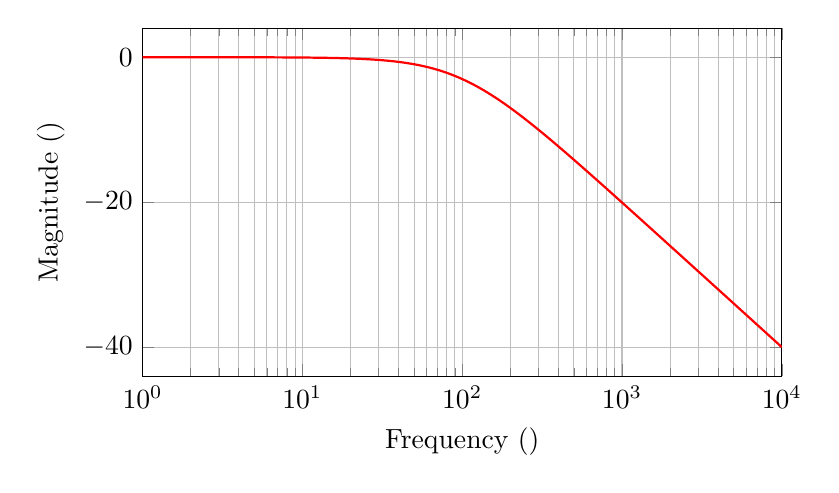
\begin{tikzpicture}
        \begin{semilogxaxis}[
            width=0.8\linewidth, height=6cm,
            xlabel={Frequency (\unit{\radian\per\second})},
            ylabel={Magnitude (\unit{\decibel})},
            xmin=1, xmax=1e4,
            grid=both,
        ]
            \addplot[thick, red, domain=1:1e4, samples=100] {-10*log10(1 + (x/100)^2)};
        \end{semilogxaxis}
    \end{tikzpicture}
    \caption{Bode magnitude plot of a first-order low-pass filter.}
    \label{fig:bode}
\end{figure}

\subsection{Circuit Diagrams}
\label{sec:circuit-diagrams}

\texttt{circuitikz} draws circuits by connecting coordinates with
components. For example, this places a resistor labelled $R$ between two
points:
\begin{center}
    \verb|\draw (0,0) to[R, l=$R$] (4,0);|
\end{center}
\Cref{fig:rc-filter} is the RC filter used in \cref{fig:bode}.

\begin{figure}[H]
    \centering
    \begin{circuitikz}[american]
        \draw (0,0) to[V, invert, l=$V_\text{in}$] (0,3)
                    to[R, l=$R$, a=\qty{10}{\kilo\ohm}] (4,3)
                    to[C, l=$C$, a=\qty{1}{\micro\farad}] (4,0)
                    -- (0,0);
        \draw (4,3) to[short, -o] (6,3) node[right] {$V_\text{out}$};
        \draw (4,0) to[short, -o] (6,0);
        \draw (0,0) node[ground] {};
    \end{circuitikz}
    \caption{RC low-pass filter.}
    \label{fig:rc-filter}
\end{figure}

\subsection{Block Diagrams}

General diagrams are drawn with \texttt{tikz}. Define a style for each
kind of node, place nodes relative to each other with \verb|right=of|, then
connect them with arrows. \Cref{fig:block} is a closed-loop control system.

\begin{figure}[H]
    \centering
    \begin{tikzpicture}[
        block/.style={draw, rectangle, minimum height=1cm, minimum width=2cm},
        sum/.style={draw, circle, inner sep=2pt},
        node distance=1.2cm,
        >=Stealth,
    ]
        \node (input) {$r(t)$};
        \node[sum, right=of input] (sum) {$\Sigma$};
        \node[block, right=of sum] (controller) {Controller};
        \node[block, right=of controller] (plant) {Plant};
        \node[right=1.5cm of plant] (output) {$y(t)$};
        \node[block, below=0.8cm of plant] (sensor) {Sensor};

        \draw[->] (input) -- node[pos=0.8, above] {$+$} (sum);
        \draw[->] (sum) -- node[above] {$e(t)$} (controller);
        \draw[->] (controller) -- node[above] {$u(t)$} (plant);
        \draw[->] (plant) -- coordinate (branch) (output);
        \draw[->] (branch) |- (sensor);
        \draw[->] (sensor) -| node[pos=0.95, right] {$-$} (sum);
    \end{tikzpicture}
    \caption{Closed-loop control system.}
    \label{fig:block}
\end{figure}

\subsection{More Code Listings}

The template defines extra listing languages in
\texttt{Code Input Perameters.tex}. Choose one with the \verb|language|
option, as in \cref{lst:gcode}.

\begin{lstlisting}[language=GCode, caption={G-code to cut a square.}, label={lst:gcode}]
G21         ; Units in millimetres
G90         ; Absolute positioning
G0 X0 Y0 Z5 ; Rapid move to start
G1 Z-1 F100 ; Plunge
G1 X20 F300 ; Cut the square
G1 Y20
G1 X0
G1 Y0
G0 Z5       ; Retract
M30         ; End of program
\end{lstlisting}

Structured Text for CODESYS uses the \verb|codesys| style instead, as in
\cref{lst:codesys}.

\begin{lstlisting}[style=codesys, caption={CODESYS Structured Text.}, label={lst:codesys}]
VAR
    StartButton AT %IX2.0 : BOOL;
    Motor       AT %QX0.0 : BOOL;
    Delay : TON;
END_VAR

Delay(IN := StartButton, PT := T#250ms);
IF Delay.Q THEN
    Motor := TRUE;
ELSE
    Motor := FALSE;
END_IF
\end{lstlisting}

Long code is better kept in its own file and pulled in with
\verb|\lstinputlisting|, as in \cref{lst:matlab-file}. Changes to the file
then appear in the report automatically.

\lstinputlisting[caption={MATLAB script loaded from \texttt{Code/step\_response.m}.}, label={lst:matlab-file}]{Code/step_response.m}

\subsection{Citations}

Cite sources with \verb|\cite{key}|, where \verb|key| is the first entry in
the \texttt{references.bib} record. Several sources can be cited at once
and the \texttt{cite} package sorts and compresses them
\cite{exampleBook,exampleConference,exampleStandard}. A single source is
cited the same way \cite{example2025}.

\cleardoublepage
